\documentclass{article}

% if you need to pass options to natbib, use, e.g.:
%     \PassOptionsToPackage{numbers, compress}{natbib}
% before loading neurips_2018

% ready for submission
%\usepackage{nips_style}

% to compile a preprint version, e.g., for submission to arXiv, add add the
% [preprint] option:
    \usepackage[preprint]{nips_style}

% to compile a camera-ready version, add the [final] option, e.g.:
     %\usepackage[final]{nips_style}

% to avoid loading the natbib package, add option nonatbib:
%\usepackage[nonatbib]{nips_style}

\usepackage[utf8]{inputenc} % allow utf-8 input
\usepackage[T1]{fontenc}    % use 8-bit T1 fonts
\usepackage{hyperref}       % hyperlinks
\usepackage{url}            % simple URL typesetting
\usepackage{booktabs}       % professional-quality tables
\usepackage{amsfonts}       % blackboard math symbols
\usepackage{nicefrac}       % compact symbols for 1/2, etc.
\usepackage{microtype}      % microtypography
\usepackage{graphicx}
\usepackage{subfig}
\usepackage{float}



\title{Deep RL literature review on multitask and transfer}

% The \author macro works with any number of authors. There are two commands
% used to separate the names and addresses of multiple authors: \And and \AND.
%
% Using \And between authors leaves it to LaTeX to determine where to break the
% lines. Using \AND forces a line break at that point. So, if LaTeX puts 3 of 4
% authors names on the first line, and the last on the second line, try using
% \AND instead of \And before the third author name.

\author{
Andrés Quintela Quintanilla - SuReLi \\
\vspace{0.1cm}\\
\textbf{Supervisor:} Emmanuel Rachelson\\
ISAE-Supaero, Toulouse
}
\begin{document}

\maketitle

\section{Introduction}
\subsection{Reinforcement Learning}
Reinforcement learning (RL) is a branch of machine learning that seeks training an agent on a given environment. The agent is able to observe the state of the environment, perform an action accordingly and receive a reward after each time-step. The objective of the agent is therefore to converge to an optimal policy that maximizes the overall reward over an episode by choosing highly-rewarded actions, but taking into account that some actions may not yield any reward at all or it may be delayed. \newline
\\
Formally, the RL problem is framed, using ideas from dynamical systems theory, as a Markov Decision Process (MDP) \cite{Sutton1998ReinforcementIntroduction}. An agent interacts with the environment as part of a sequence of discrete time-steps by selecting an action, $A_{t}$, depending on the environment's state, $S_{t}$. This decision brings the agent to a new state, $S_{t+1}$, and generates a reward, $R_{t+1}$.
This gives rise to a trajectory through the state-action space ( $\mathcal{S} \times \mathcal{A}$ ) governed by the state-transition probabilities \citep{Sutton1998ReinforcementIntroduction}:
\begin{equation}
    p(s'|s,a) = \Pr \{ S_{t+1}|S_{t}, A_{t} \}
\end{equation}
Reward is accumulated along the duration of an episode (finite sequence of discrete time-steps until a terminal state is reached \citep{Sutton1998ReinforcementIntroduction}) and this \textit{accumulated reward} is a measure of the performance of the agent during this episode. The agent pursuits the goal of maximizing the accumulated reward by choosing the best possible actions, and hence all RL algorithms involve evaluating how good it is to be in a given state. \\ 
The agent's behaviour is governed by a policy, $\pi (a|s)$, a probabilistic mapping of actions to take for each state, which is modified during learning in order to achieve the maximum possible accumulated reward.
The \textit{value function} evaluates how good it is to be in a given state and is defined as \citep{Sutton1998ReinforcementIntroduction}:
\begin{equation}
    v_{\pi}(s)=\mathop{\mathbb{E}}_{\pi} \Big [ \sum_{k=0}^{\infty} \gamma^k R_{t+k+1} \big | S_{t}=s \Big]
\end{equation}
where $\gamma$ is the discount factor used to ensure convergence on non-finite MDPs.\\
In the same fashion, the action-value function, $q$, is defined as the expected return starting from state $s$, taking action $a$ thereafter following policy $\pi$ \cite{Sutton1998ReinforcementIntroduction}.
\begin{equation}
    q_{\pi}(s)=\mathop{\mathbb{E}}_{\pi} \Big [ \sum_{k=0}^{\infty} \gamma^k R_{t+k+1}\big | S_{t}=s ,A_{t}=a \Big ]
\end{equation}

The agent's ultimate goal, achieving maximum accumulated reward is achieved by finding the best policy, \textit{the optimal policy} ($v_{*}$), by means of the Bellman optimality equation \citep{Sutton1998ReinforcementIntroduction}:
\begin{equation}
    v_{*}(s)=\max_{a \in \mathcal{A}(s)} q_{\pi_{*}}(s,a)
\end{equation}
which implies the estimation of the \textit{state-action value function} (or \textit{state value function}). This is necessary in almost all RL algorithms and can be achieved by means of algorithms such as the Monte Carlo methods, Temporal Difference, Q-Learning and many others.
\subsection{Deep Reinforcement Learning (DRL)}
The increasing complexity of RL problems and the development of neural networks lead to the development of DRL. DRL tackles the limitation of value function estimation and policy search in high-dimensional state and action spaces with the introduction of neural networks as function approximators \citep{Arulkumaran2017ALearning}. This has allowed for the scaling up prior RL algorithms into high-dimensional problems, such as those obtaining the state representation directly from visual inputs by means of convolutional neural networks (CNNs) \citep{Arulkumaran2017ALearning}. The first breakthrough in DRL was achieved by the Deep-Q Network algorithm (DQN) \citep{MnihPlayingLearning} by successfully attaining superhuman performance on several Atari 2600 games with the sole input of raw pixels.
\section{Motivation}
In the past years, many algorithms have been developed that surpass the benchmarks achieved by the DQN algorithm in \citep{MnihPlayingLearning} by introducing different variations \citep{Bellemare2017ALearning},\citep{Mnih2015Human-levelLearning}, \citep{vanHasselt2015DeepQ-learning},\citep{Wang2015DuelingLearning}. All this improvements were combined in the \textit{Rainbow} algorithm \citep{Hessel2017Rainbow:Learning}, which achieved state of the art performance on the Arcade Learning Environment (ALE)\citep{Bellemare2013TheAgents}. However, the main limitation of these approaches is the fact that the network needs to be trained separately for every task, which involves processing, in most cases, hundreds of millions of frames.\\
\newline 
Multitask and transfer RL seek to solve these scalability issues by enabling knowledge reuse in the initial fases of learning in a novel task. In short, \textit{multitasking} agents, who's objective is to solve multiple related or unrelated problems, seek to \textit{transfer} previously acquired knowledge on different tasks to facilitate the learning of a novel task. This enables faster training and smaller computational cost.\\
\newline
This branch of RL presents several problems and limitations, some of which we seek to overcome in this project. Related work in this field has achieved several advancements recently, successfully training agents that can perform reasonably well on several related Atari games and on different tasks with similar environments.\\
\newline
Our work seeks to develop an agent that is able to learn how to play many Atari games using a common neural network as a action-value function approximator. This agent should be able to adapt to a new game swiftly, reusing previous knowledge and requiring minimal training.\\
%In the continuing sections the state of the art in these will be analyzed and related to the purposes of this project.
\section{Multitask and transfer RL}
\subsection{Literature review}
During the past years, multitask and transfer learning have developed at a great pace, but they are far from reaching maturity. Several breakthroughs have been achieved since the introduction of policy distillation and deep multitasking in the RL domain ( \citep{RusuPOLICYDISTILLATION}, \citep{Parisotto2015Actor-Mimic:Learning})  many based, to some extent, in the ideas presented on these papers.\\
\newline
\textit{Distillation} is a method to transfer knowledge from a teacher network to a student one in order to significantly reduce its size and complexity \citep{RusuPOLICYDISTILLATION}. This same idea, applied to policies, can be used to combine multiple reinforcement learning policies more effectively, process which is known as \textit{policy distillation}. Policies are more effectively combined thanks to the fact that they are compressed and refined during distillation, throwing evidence that distillation is a general principle for model regularization as \textit{Rusu et al.} concluded. In their work, they also proposed a structure in which the common multitask agent learnt from several expert DQN teachers sharing all the hyperparameters except the output layer, namely the \textit{controller}, which was task-specific. Their agent was trained by alternating an episode from each task and was able to obtain a $90\%$ mean performance on 10 ALE game compared to single DQN agents.\\
\newline
Following the same ideas, \textit{Teh et al.} \citep{Teh2017Distral:Learning} proposed a novel framework for transfer and multitasking which they reffered to as \textit{Distral} (DIStil and TRAnsfer Learning), in which they exploit \textit{policy distillation} and model \textit{regularization}. Their algorithm seeks to train a shared policy which \textit{distills} behaviours from task-specific experts, as shown on Figure \ref{fig:high -level}. The distilled policy is then used to regularize the task specific policies towards the shared policy by means of Kullback-Leibler (KL) divergence so that it learns to be the centroid in the space of policies. In opposition to the multi-tasking policy distillation algorithm proposed by \textit{Rusu et al.}, the Distral framework enables not only teacher-student transfer but also inter-teacher transfer thanks to the imposed KL divergence regularization. The algorithm was tested in several DeepMindLab environments, which are three-dimensional spaces of higher complexity than Atari games, and compared to a multitask A3C agent. The results showed that the Distral algorithm learnt faster, achieving a higher score while also being more stable.\\
\begin{figure}[!ht]
     \subfloat[Illustration of the Distral Framework]{%
       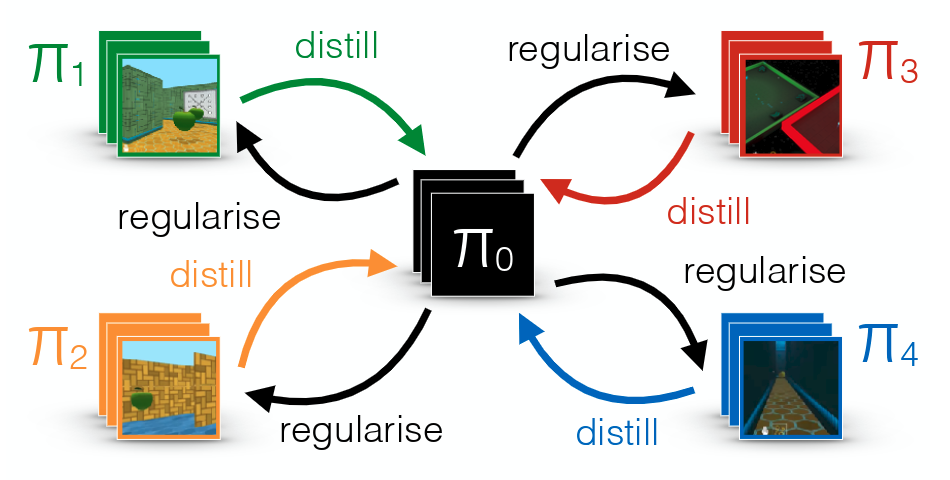
\includegraphics[width=0.45\textwidth]{figs/distral.png}
     }
     \hfill
     \subfloat[Multi-task pollicy distillation architecture]{%
       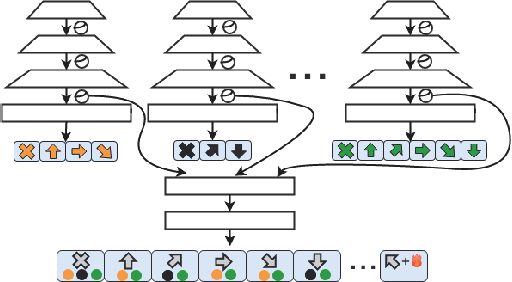
\includegraphics[width=0.45\textwidth]{figs/transfer.png}
     }
     \caption{The figures above are high-level representations of the algorithms presented and were borrowed from \citep{Teh2017Distral:Learning} and \citep{YinKnowledgeReplay} respectively.}
     \label{fig:high -level}
\end{figure}
\newline
In parallel to the developement of the \textit{policy distillation} framework, \textit{Parisotto et al.} \citep{Parisotto2015Actor-Mimic:Learning} proposed a novel approach for multi-task and transfer learning which they named \textit{Actor-mimic} (AM). This autonomous agent is capable of learning how to behave in multiple tasks simultaneously while generalizing its knowledge to new domains by means of model compression techniques. The \textit{Actor-mimic} agent is trained from experts on each of the tasks, thus following the same principle as \citep{RusuPOLICYDISTILLATION} and \citep{Teh2017Distral:Learning}, but differs on the way it is trained. 
The learning of the AM agent is driven by the combination of two objective functions, the policy regression and the feature regression objetive. The first of these two is achieved by first transforming the expert networks Q-value output by means of a \textit{softmax} and then using this to define the cross-entropy between the multitask AM agent and each respective expert. This bounding of the Q-values by the \textit{softmax} function diminishes the effects of the different scales of Q-functions and thus leads to higher stability in learning. The second objective function, feature regression, is used to train the AM network with an additional loss function. This loss is defined between the feature (pre-output) layer of the AM network and the feature layer of the experts. \textit{Parisotto et al.} succesfully proved that adding this loss term increases the performace of transfer in some tasks. The first objective can be seen as the 'what' in an instruction while the second represents the 'why'.\\ 
The AM agent was tested on 8 Atari games maintaining the same network size and structure for the AM and the DQN experts in order to asses multitasking. \textit{Parisotto et al.} noticed that the AM network network reached close-to-expert performance much faster compared to the expert DQNs and achieved a higher mean reward on 3 of them. Setting the focus on transfer learning, the experiment was repeated increasing the AM network size, which enabled the number of games to be increased to 13. This network was trained and then used as weight initialization for DQNs on the source tasks. This showed a significant increment in learning speed proving that features learned in some tasks can be transferred to others if they are similar to some extent.\\

Furthermore, \textit{Yin et al.} \citep{YinKnowledgeReplay} set as an objective to address the main flaws of the above proposed strategies: these architectures involve a great number of hyperparameters and hence are computationally expensive to train, the multi-task network does not always perform as good as the experts and, finally, sampling from the different task is not done sufficiently efficiently.\\
They developed a new multi-task policy distillation architecture in which each task preserves its own convolutional filters while sharing a set of fully-connected layers, such as shown in Figure \ref{fig:high -level} b). The output layer is hence formed of the combination of all the possible actions for all the tasks. As shown by \textit{Rusu et al.}, matching the q-value distribution is more effective so the multi-task student network was trained using KL divergence and matching the output distributions from the student and teacher networks. As they observed, keeping the convolutional filters task-specific prevents negative transfer.\\
On the other hand, \textit{Yin et al.} also proposed a novel approach to memory sampling which they named \textit{hierachical prioritized experience replay}. This method is an improved version of \textit{prioritized experience replay} \citep{Schaul2015PrioritizedReplay} which samples experiences according to the magnitude of their TD error, which involves that the origial state distribution can not be preserved \cite{YinKnowledgeReplay}. This novel method divides the memory samples into several partitions, each partition covering a different part of the state distribution, and the samples inside each partition are prioritized according to their KL divergence absolute value.\\
This novel architecture was tested on 10 Atari games and compared to policy distillation and Actor-critic algorithms, as shown on Figure \ref{fig:comparison}. Not only training time was significantly faster compared to the other two, but it also obtained higher mean performance on all 10 games compared to their corresponding teacher DQN.\\
\begin{figure}[H]
    \centering
    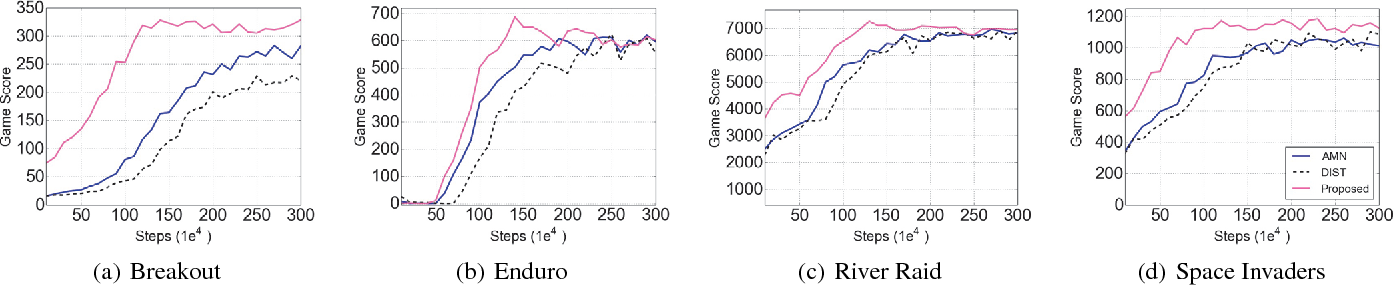
\includegraphics[width=\textwidth]{figs/comparison.png}
    \caption{Figured borrowed from \citep{YinKnowledgeReplay} comparing three multi-task frameworks evaluated on different Atari games. 'AMN' stands for the algorithm developed by \textit{Parisotto et al.}, 'DIST' stands for \textit{policy distillation} by \textit{Rusu et al.} and 'proposed' stands for \textit{Yin et al.} approach.}
    \label{fig:comparison}
\end{figure}
\subsection{Our algorithm}
As reviewed above, many have attempted to address the multi-tasking problem in RL by different means and impressive milestones have been achieved, but this field's developement is still relatively immature. Transfer achieved between tasks is limited and difficult to quantify and understand. Furthermore, training times are still long and networks require a vast number of hyperparameters.\\ 
In order to confront these issues, we propose to abandon the idea of a common network that can solve a large number of tasks keeping the same hyperparameters. Instead, we seek to develop an algorithm that is able to train a network in several tasks, transferring efficiently previous knowledge to novel tasks to reduce training times while only requiring a minimal fine-tuning previous to executing a specific task. This can be seen as finding a set of hyperparameters for the common core of the multi-task network which require minimal fine-tuning in order to execute any task at expert level. Thus we intend to implement a multi-task agent that exploits similarities between tasks in different levels via transfer while keeping the size of the network to its minimum. We believe allowing for a fine-tuning will enable us to decrease the network size significantly compared to the approaches presented in the previous section, making our algorithm more functional, vastly reducing training times. We also believe, by this same reason, that transfer of knowledge between tasks is going to be favored as the network will be able to generalize information which is common to several tasks at a higher level, working as a cortex from which task-specific behaviours can be extracted via the combination of task-specific output layers and fine-tuning.\\

\section{The continual learning problem}
\subsection{Why is this a problem?}
When considering the approach we have proposed in the section above, consolidating the task-specific information in the network arises as a clear limitation, as the optimal weights for one task may not be of use at all for the following one. This is known as \textit{catastrophic forgetting}, the tendency of neural networks to perturb previous knowledge when new, unrelated one is acquired. In the supervised learning problem, this would be the case when a network trained to recognise one specific class is trained to recognise a different one, it will most likely overwrite its weights in order to predict the second task. In our case, as we use a neural networks to approximate a state-action value function which is different for each task, we need to ensure new information is consolidated properly so that previously learnt tasks are not perturbed. From another point of view, we need to ensure that the new hyperparameters are as close to each other as possible in order to require minimal fine-tuning to perform at expert level on any. This obvious limitation lead to search for inspiration in the continual learning literature.

\subsection{Literature overview}
Continual learning is the ability to learn tasks in a sequential fashion without perturbing previous knowledge and it is a crucial matter towards the development of artificial intelligence. Due to the fact that a great number of artificial neural network models suffer from catastrophic forgetting, which impedes continual learning, several approaches have sought to solve this issue.\\
\newline
\textit{Robins} \citep{RobinsConsolidationBrain} proposed the use of \textit{rehearsal} and \textit{pseudorehearsal} mechanisms to alleviate this effect. These mechanisms interleave previously learnt items while new items are introduced. \textit{Rehearsal} uses real transitions drawn for a memory buffer meanwhile \textit{pseudorehearsal} uses \textit{pseudo-transitions} generated by passing a random input vector through the network. The main drawback of this solution is that it can not be applied when information is received sequentially and can not be shuffled. At the same time, if old samples can be introduced during learning, this would require to keep a memory buffer for each task which leads to large memory requirements.\\
Other approaches can be classified into regularization approaches, dynamic architectures and dual memory-learning systems \citep{Parisi2018ContinualReview}.\\
\newline
Regularization approaches seek to alleviate catastrophic forgetting by imposing limits on the update of neural weights. \textit{Kirkpatrick et al.} \citep{Kirkpatrick2017OvercomingNetworks.} proposed a framework called Elastic Weight Consolidation (EWC) which slows down learning on some weights depending on how important they are to previous tasks. In order to do this, they constrain parameters to stay close to previous values. This can be seen, as they explain, as linking the old weights to the new ones with a spring whose stiffness depends on the importance each weight has towards the performance on previous tasks. Assessing the relevance of each weight is done by means of an approximation using a Gaussian distribution with a mean given by the old previous tasks parameters and a diagonal precision given by the Fischer's information matrix. EWC was implemented in a regular DQN and tested on 10 Atari games. This algorithm managed to learn  10 different Atari games sequentially but however it did not reach single DQN expert scores. \textit{Zenke et al.} \citep{Zenke2017ContinualIntelligence} suggested a very similar approach but changed the way in which the weight importance is determined. These approaches alleviate catastrophic forgetting with a compromise of task performance but have scalability issues, as performance decreases considerably as the number of tasks is increased.\\
\newline
Dynamic architectures allocate novel neural resources whenever  new tasks or classes are learnt. However, this is not very interesting in our application as the covolutional nets used in RL algorithms are already very large and this would lead to scalability issues. Thus, we will not consider this approach as we seek to develop a functional algorithm with the minimal network size. In the other hand, it may be useful to consider, in a future stage, the possibility of subdividing learning in two stages: a first one where new neural resources are allocated to facilitate assimilation of novel tasks and a second one in which this knowledge is compressed or \textit{distilled} to extract the useful information.\\
\newline
Dual-memory systems propose the use of complementary networks that separate the functions of memorization and generalization. This is inspired by the \textit{complementary learning systems} theory by \textit{McClelland et al.}\citep{McClelland1995WhyMemory.} which explains how learning works in the mammalian brain. They showed that the mammalian brain uses two stuctures in the learning process. The first one, the hippocampus, is used for short term memory (rapid learning) while the neocortex, the second one, is used for long term memory. \textit{Robins} then complemented this theory suggesting that information is slowly consolidated in off-line phases in the neocortex, using \textit{pseudorehearsal}. This idea can be exploited in neural networks by using separate networks for novel knowledge assimilation and for knowledge consolidation, although advances have not been made on the RL domain.\\
\newline
Futhermore, besides the different approaches to the continual learning problem, \textit{Achille et al.} \citep{Achille2017CriticalNetworks} showed how the initial rapid learning phase of a neural networks is critical to neural ressource allocation, which plays a key role in the final performance of the network.
\section{Conclusion}

Addressing directly the continual learning problem in our way to obtaining the proposed algorithm is a key step towards its completion and marks a difference between the approaches presented in section 3 and our own. The ideas introduced in EWC \citep{Kirkpatrick2017OvercomingNetworks.} and the concepts of \textit{pseudorehearsal} and dual-memory systems are going to play a significant role towards its accomplishment while the understanding of the state of the art in this matter has been crucial towards fitting our idea inside the multitask and transfer landscape. 




\newpage
\bibliographystyle{plain} % We choose the "plain" reference style
\bibliography{references.bib} % Entries are in the "refs.bib" file
\end{document}